\documentclass[tikz]{standalone}
\usepackage{tikz}
\usetikzlibrary{shapes.geometric}
\usetikzlibrary{calc}

\begin{document}
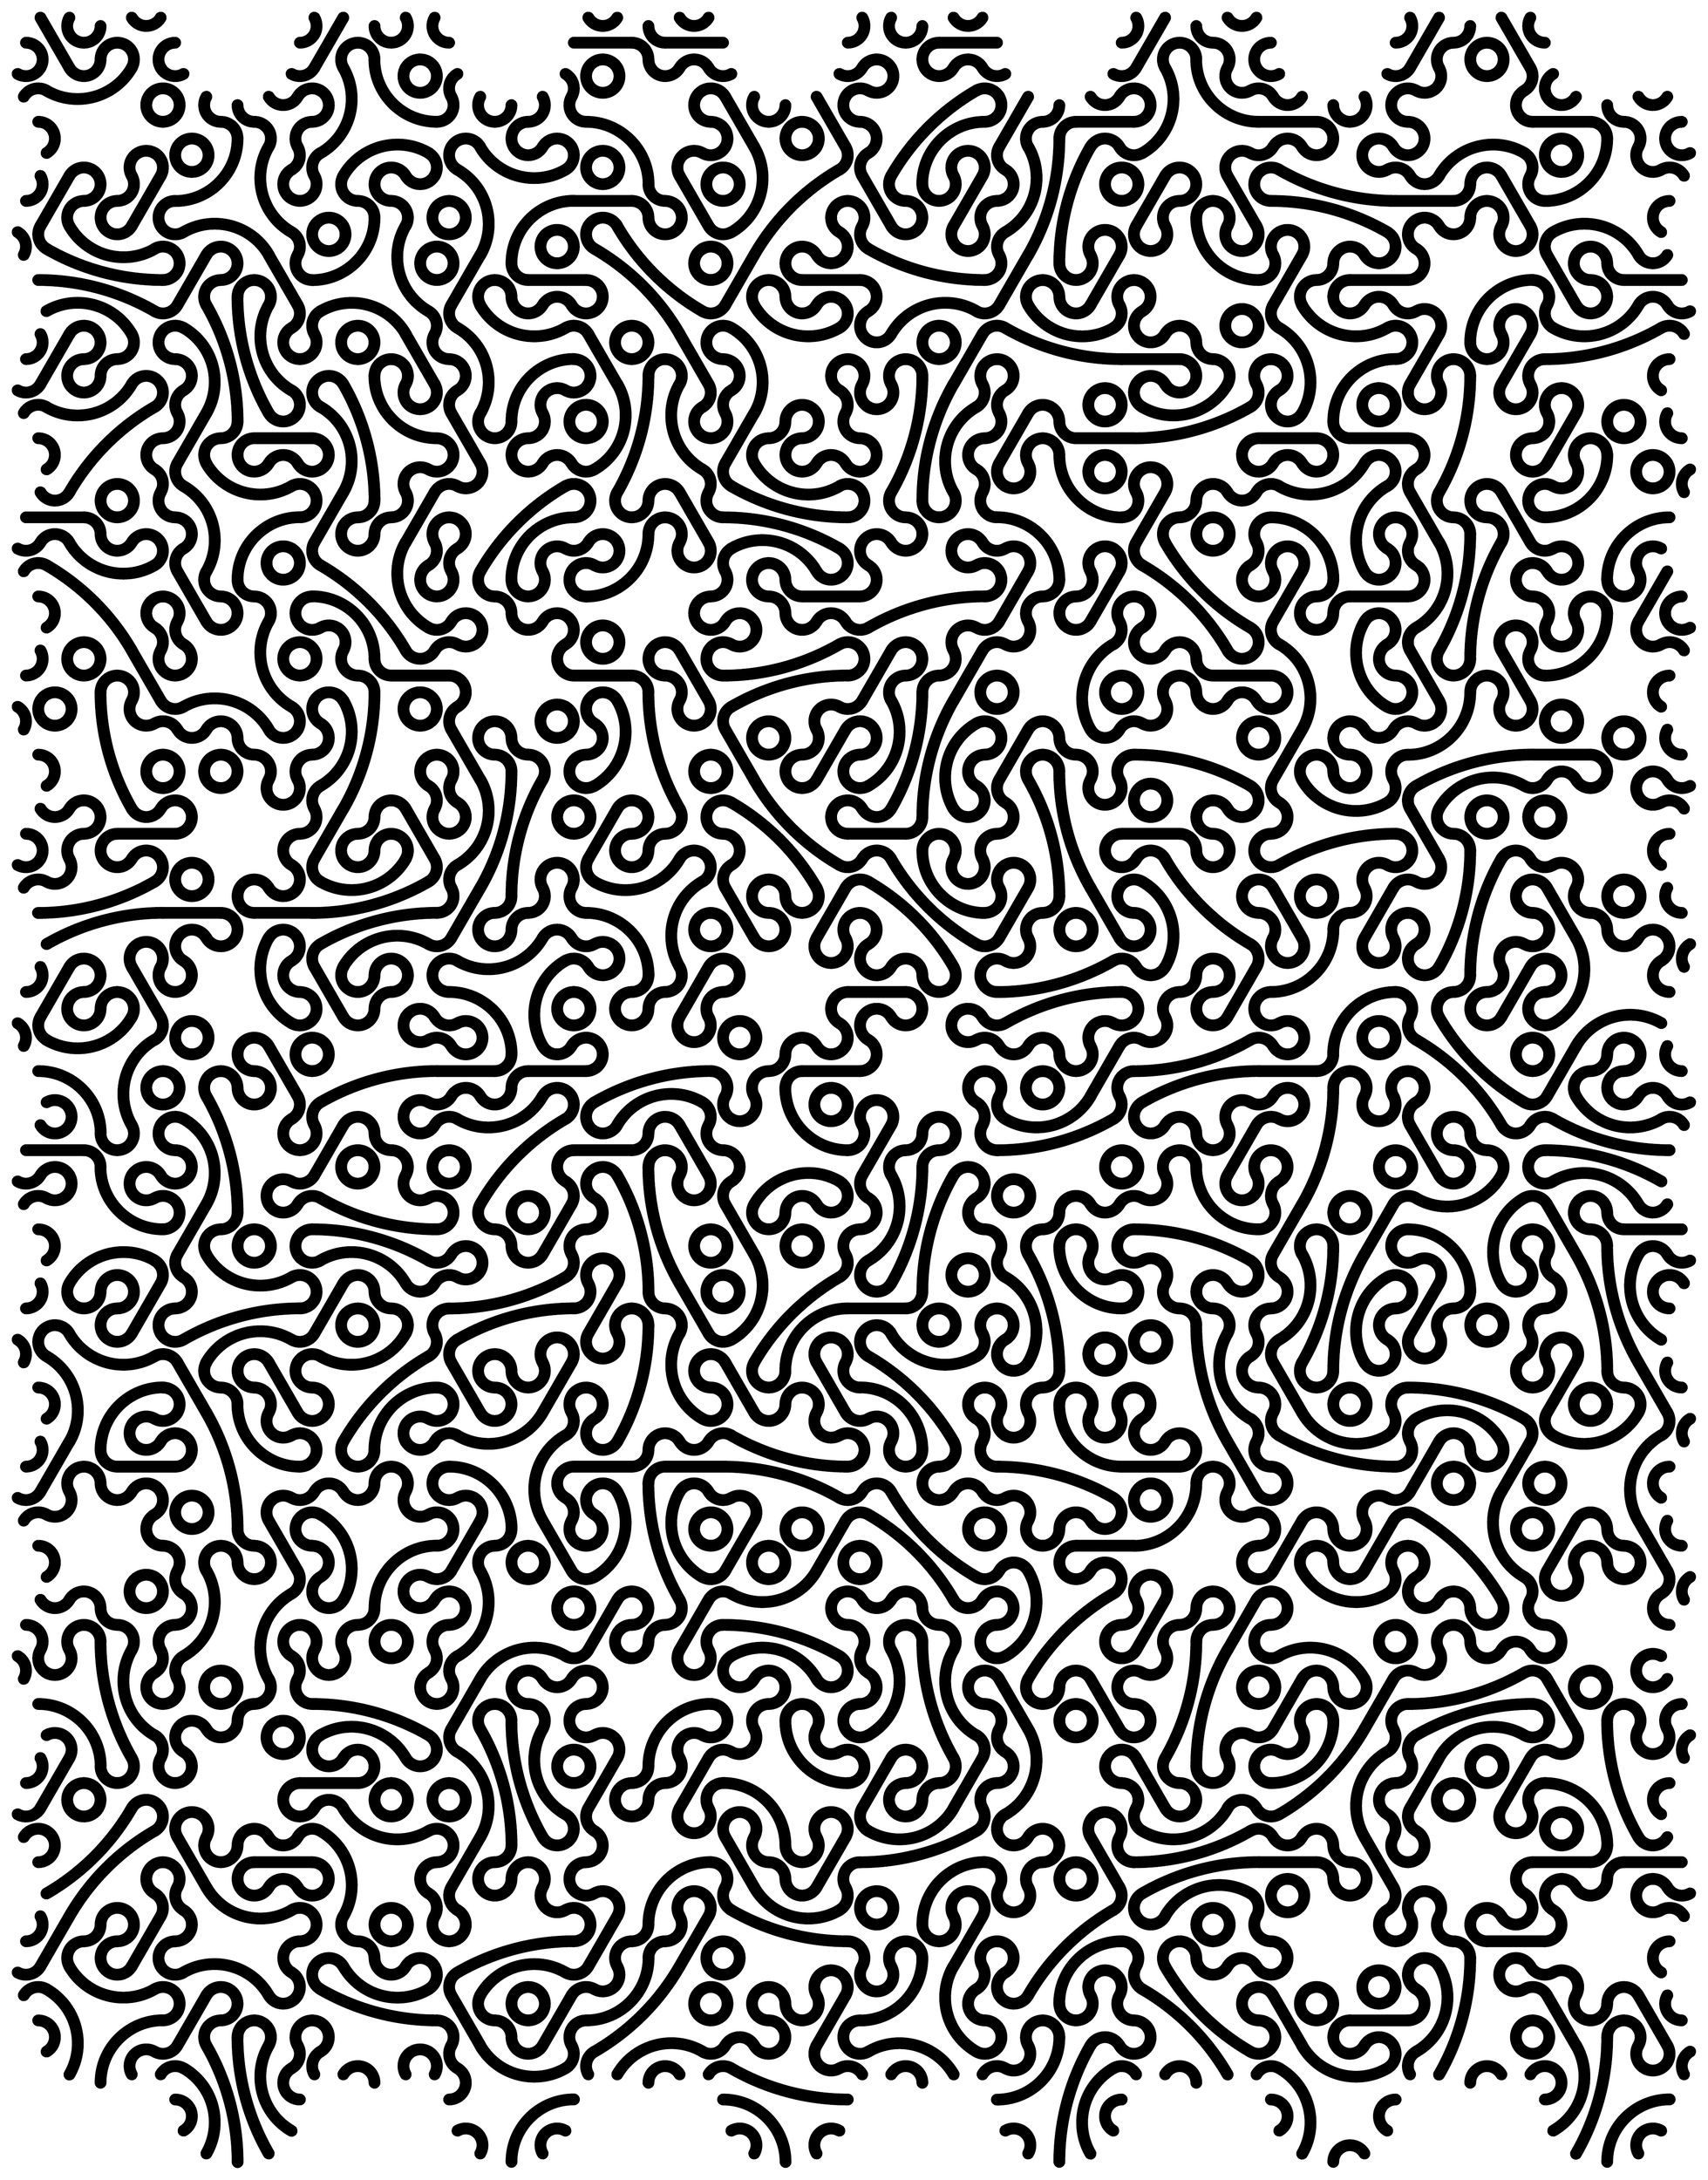
\begin{tikzpicture}
  \newcommand\n{12}

  \foreach \a [
    evaluate=\bmin using {int(-\a/2)},
    evaluate=\bmax using {\n + \bmin},
  ] in {1,...,\n} {
    \foreach \b [
      evaluate=\x using {(3*sqrt(3)+3)/2*\a},
      evaluate=\y using {(3+sqrt(3))*(\b + \a/2)},
      evaluate=\r using {random(0,167)},
      evaluate=\c using {(\x+\y)*9/\n},
    ] in {\bmin,...,\bmax} {
      \node at (\x,\y) (dodecagonCenter) {};
      % 3.85 is an approximation of 3.84370 that takes into account the size of the padding.
      \node[minimum size=3.85 cm, regular polygon, regular polygon sides=12] at (\x,\y) (p\a\b) {};
      % \draw[ultra thin, orange] let
      %   \p{1}=($(p\a\b.corner 1)$), % Top
      %   \p{2}=($(p\a\b.corner 2)$), % SW
      %   \p{3}=($(p\a\b.corner 3)$), % SE
      %   \p{4}=($(p\a\b.corner 4)$), % SE
      %   \p{5}=($(p\a\b.corner 5)$), % SE
      %   \p{6}=($(p\a\b.corner 6)$), % SE
      %   \p{7}=($(p\a\b.corner 7)$), % SE
      %   \p{8}=($(p\a\b.corner 8)$), % SE
      %   \p{9}=($(p\a\b.corner 9)$), % SE
      %   \p{10}=($(p\a\b.corner 10)$), % SE
      %   \p{11}=($(p\a\b.corner 11)$), % SE
      %   \p{12}=($(p\a\b.corner 12)$), % SE
      % in
      %   (\p{1}) \foreach \z in {2,...,12} {-- (\p{\z})} -- cycle
      %   \foreach \z in {1,...,12} {(\p{\z}) circle (0.01)}
      % ;
      \ifnum \r < 12 {
        % Type I
        \draw[line width=10, line cap=round] let
          \p{1}  = ($(p\a\b.corner 1)!0.5!(p\a\b.corner 2)$), % Top
          \p{3}  = ($(p\a\b.corner 3)!0.5!(p\a\b.corner 4)$), %
          \p{5}  = ($(p\a\b.corner 5)!0.5!(p\a\b.corner 6)$),
          \p{7}  = ($(p\a\b.corner 7)!0.5!(p\a\b.corner 8)$),
          \p{9}  = ($(p\a\b.corner 9)!0.5!(p\a\b.corner 10)$),
          \p{11} = ($(p\a\b.corner 11)!0.5!(p\a\b.corner 12)$),
        in [rotate around={30*\r:(dodecagonCenter)}]
          (\p{1})  arc (0:-150:0.5)
          (\p{3})  arc (60:-90:0.5)
          (\p{5})  arc (120:-30:0.5)
          (\p{7})  arc (180:30:0.5)
          (\p{9})  arc (240:90:0.5)
          (\p{11}) arc (300:150:0.5)
        ;
      } \else {
      \ifnum \r < 24 {
        % Type 2
        \draw[line width=10, line cap=round] let
          \p{1}  = ($(p\a\b.corner 1)!0.5!(p\a\b.corner 2)$), % Top
          \p{3}  = ($(p\a\b.corner 3)!0.5!(p\a\b.corner 4)$), %
          \p{5}  = ($(p\a\b.corner 5)!0.5!(p\a\b.corner 6)$),
          \p{7}  = ($(p\a\b.corner 7)!0.5!(p\a\b.corner 8)$),
          \p{9}  = ($(p\a\b.corner 9)!0.5!(p\a\b.corner 10)$),
          \p{11} = ($(p\a\b.corner 11)!0.5!(p\a\b.corner 12)$),
        in [rotate around={30*\r:(dodecagonCenter)}]
          (\p{1})  arc (0:-150:0.5)
          (\p{3})  arc (240:330:1.87) % Radius is a guess.
          (\p{5})  arc (120:-30:0.5)
          (\p{7})  arc (180:30:0.5)
          (\p{9})  arc (240:90:0.5)
          (\p{11}) arc (300:270:6.98) % Radius is a guess
        ;
      } \else {
      \ifnum \r < 36 {
        % Type 3
        \draw[line width=10, line cap=round] let
          \p{1}  = ($(p\a\b.corner 1)!0.5!(p\a\b.corner 2)$), % Top
          \p{3}  = ($(p\a\b.corner 3)!0.5!(p\a\b.corner 4)$), %
          \p{5}  = ($(p\a\b.corner 5)!0.5!(p\a\b.corner 6)$),
          \p{7}  = ($(p\a\b.corner 7)!0.5!(p\a\b.corner 8)$),
          \p{9}  = ($(p\a\b.corner 9)!0.5!(p\a\b.corner 10)$),
          \p{11} = ($(p\a\b.corner 11)!0.5!(p\a\b.corner 12)$),
        in [rotate around={30*\r:(dodecagonCenter)}]
          (\p{1})  arc (0:-90:1.87)
          (\p{3})  arc (-120:30:0.5)
          (\p{5})  arc (120:-30:0.5)
          (\p{7})  arc (180:30:0.5)
          (\p{9})  arc (240:90:0.5)
          (\p{11}) arc (300:150:0.5)
        ;
      } \else {
      \ifnum \r < 48 {
        % Type 4
        \draw[line width=10, line cap=round] let
          \p{1}  = ($(p\a\b.corner 1)!0.5!(p\a\b.corner 2)$), % Top
          \p{3}  = ($(p\a\b.corner 3)!0.5!(p\a\b.corner 4)$), %
          \p{5}  = ($(p\a\b.corner 5)!0.5!(p\a\b.corner 6)$),
          \p{7}  = ($(p\a\b.corner 7)!0.5!(p\a\b.corner 8)$),
          \p{9}  = ($(p\a\b.corner 9)!0.5!(p\a\b.corner 10)$),
          \p{11} = ($(p\a\b.corner 11)!0.5!(p\a\b.corner 12)$),
        in [rotate around={30*\r:(dodecagonCenter)}]
          (\p{1})  arc (0:-150:0.5)
          (\p{3})  arc (240:330:1.87) % Radius is a guess.
          (\p{5})  arc (120:90:6.98)
          (\p{7})  arc (0:150:0.5)
          (\p{9})  arc (60:210:0.5)
          (\p{11}) arc (300:270:6.98) % Radius is a guess
        ;
      } \else {
      \ifnum \r < 60 {
        % Type 5
        \draw[line width=10, line cap=round] let
          \p{1}  = ($(p\a\b.corner 1)!0.5!(p\a\b.corner 2)$), % Top
          \p{3}  = ($(p\a\b.corner 3)!0.5!(p\a\b.corner 4)$), %
          \p{5}  = ($(p\a\b.corner 5)!0.5!(p\a\b.corner 6)$),
          \p{7}  = ($(p\a\b.corner 7)!0.5!(p\a\b.corner 8)$),
          \p{9}  = ($(p\a\b.corner 9)!0.5!(p\a\b.corner 10)$),
          \p{11} = ($(p\a\b.corner 11)!0.5!(p\a\b.corner 12)$),
        in [rotate around={30*\r:(dodecagonCenter)}]
          (\p{1})  arc (0:-150:0.5)
          (\p{3})  arc (240:330:1.87) % Radius is a guess.
          (\p{5})  arc (120:90:6.98) % Radius is a guess
          (\p{7})  arc (180:30:0.5)
          (\p{9})  arc (60:150:1.87) % Radius is a guess.
          (\p{11}) arc (300:270:6.98) % Radius is a guess
        ;
      } \else {
      \ifnum \r < 72 {
      % Type 6
      \draw[line width=10, line cap=round] let
        \p{1}  = ($(p\a\b.corner 1)!0.5!(p\a\b.corner 2)$), % To
        \p{3}  = ($(p\a\b.corner 3)!0.5!(p\a\b.corner 4)$), %
        \p{5}  = ($(p\a\b.corner 5)!0.5!(p\a\b.corner 6)$),
        \p{7}  = ($(p\a\b.corner 7)!0.5!(p\a\b.corner 8)$),
        \p{9}  = ($(p\a\b.corner 9)!0.5!(p\a\b.corner 10)$),
        \p{11} = ($(p\a\b.corner 11)!0.5!(p\a\b.corner 12)$),
      in [rotate around={30*\r:(dodecagonCenter)}]
        (\p{1})  arc (0:-150:0.5)
        (\p{3})  arc (240:330:1.87) % Radius is a guess.
        (\p{5})  arc (-60:90:0.5)
        (\p{7})  arc (180:30:0.5)
        (\p{9})  arc (60:150:1.87) % Radius is a guess.
        (\p{11})  arc (120:270:0.5)
      ;
      } \else {
      \ifnum \r < 84 {
        % Type 7
        \draw[line width=10, line cap=round] let
          \p{1}  = ($(p\a\b.corner 1)!0.5!(p\a\b.corner 2)$), % Top
          \p{3}  = ($(p\a\b.corner 3)!0.5!(p\a\b.corner 4)$), %
          \p{5}  = ($(p\a\b.corner 5)!0.5!(p\a\b.corner 6)$),
          \p{7}  = ($(p\a\b.corner 7)!0.5!(p\a\b.corner 8)$),
          \p{9}  = ($(p\a\b.corner 9)!0.5!(p\a\b.corner 10)$),
          \p{11} = ($(p\a\b.corner 11)!0.5!(p\a\b.corner 12)$),
        in [rotate around={30*\r:(dodecagonCenter)}]
          (\p{1}) arc (-180:-30:0.5)
          (\p{3})  arc (-120:30:0.5)
          (\p{5})  arc (120:90:6.98) % Radius is a guess
          (\p{7})  arc (0:150:0.5)
          (\p{9})  arc (60:210:0.5)
          (\p{11}) arc (300:270:6.98) % Radius is a guess
        ;
      } \else {
      \ifnum \r < 96 {
        % Type 8
        \draw[line width=10, line cap=round] let
          \p{1}  = ($(p\a\b.corner 1)!0.5!(p\a\b.corner 2)$), % Top
          \p{3}  = ($(p\a\b.corner 3)!0.5!(p\a\b.corner 4)$), %
          \p{5}  = ($(p\a\b.corner 5)!0.5!(p\a\b.corner 6)$),
          \p{7}  = ($(p\a\b.corner 7)!0.5!(p\a\b.corner 8)$),
          \p{9}  = ($(p\a\b.corner 9)!0.5!(p\a\b.corner 10)$),
          \p{11} = ($(p\a\b.corner 11)!0.5!(p\a\b.corner 12)$),
        in [rotate around={30*\r:(dodecagonCenter)}]
          (\p{1})  arc (0:-150:0.5)
          (\p{3})  arc (60:-90:0.5)
          (\p{5})  arc (120:90:6.98) % Radius is a guess
          (\p{7})  arc (0:150:0.5)
          (\p{9})  arc (60:210:0.5)
          (\p{11}) arc (300:150:0.5)

        ;
      } \else {
      \ifnum \r < 108 {
        % Type 9
        \draw[line width=10, line cap=round] let
          \p{1}  = ($(p\a\b.corner 1)!0.5!(p\a\b.corner 2)$), % Top
          \p{3}  = ($(p\a\b.corner 3)!0.5!(p\a\b.corner 4)$), %
          \p{5}  = ($(p\a\b.corner 5)!0.5!(p\a\b.corner 6)$),
          \p{7}  = ($(p\a\b.corner 7)!0.5!(p\a\b.corner 8)$),
          \p{9}  = ($(p\a\b.corner 9)!0.5!(p\a\b.corner 10)$),
          \p{11} = ($(p\a\b.corner 11)!0.5!(p\a\b.corner 12)$),
        in [rotate around={30*\r:(dodecagonCenter)}]
          (\p{1})  arc (0:-150:0.5)
          (\p{3})  arc (240:330:1.87) % Radius is a guess.
          (\p{5})  arc (120:-30:0.5)
          (\p{7})  arc (180:90:1.87)
          (\p{9})  arc (60:210:0.5)
          (\p{11}) arc (300:270:6.98) % Radius is a guess
        ;
      } \else {
      \ifnum \r < 120 {
        % Type 10
        \draw[line width=10, line cap=round] let
          \p{1}  = ($(p\a\b.corner 1)!0.5!(p\a\b.corner 2)$), % Top
          \p{3}  = ($(p\a\b.corner 3)!0.5!(p\a\b.corner 4)$), %
          \p{5}  = ($(p\a\b.corner 5)!0.5!(p\a\b.corner 6)$),
          \p{7}  = ($(p\a\b.corner 7)!0.5!(p\a\b.corner 8)$),
          \p{9}  = ($(p\a\b.corner 9)!0.5!(p\a\b.corner 10)$),
          \p{11} = ($(p\a\b.corner 11)!0.5!(p\a\b.corner 12)$),
        in [rotate around={30*\r:(dodecagonCenter)}]
          (\p{1})  arc (0:-150:0.5)
          (\p{3})  arc (240:330:1.87) % Radius is a guess.
          (\p{5})  arc (120:30:1.87)
          (\p{7})  arc (0:150:0.5)
          (\p{9})  arc (240:90:0.5)
          (\p{11}) arc (300:270:6.98) % Radius is a guess
        ;
      } \else {
      \ifnum \r < 132 {
        % Type 11
        \draw[line width=10, line cap=round] let
          \p{1}  = ($(p\a\b.corner 1)!0.5!(p\a\b.corner 2)$), % Top
          \p{3}  = ($(p\a\b.corner 3)!0.5!(p\a\b.corner 4)$), %
          \p{5}  = ($(p\a\b.corner 5)!0.5!(p\a\b.corner 6)$),
          \p{7}  = ($(p\a\b.corner 7)!0.5!(p\a\b.corner 8)$),
          \p{9}  = ($(p\a\b.corner 9)!0.5!(p\a\b.corner 10)$),
          \p{11} = ($(p\a\b.corner 11)!0.5!(p\a\b.corner 12)$),
        in [rotate around={30*\r:(dodecagonCenter)}]
          (\p{1}) arc (-180:-30:0.5)
          (\p{3})  arc (-120:30:0.5)
          (\p{5})  arc (120:-30:0.5)
          (\p{7})  arc (180:90:1.87)
          (\p{9})  arc (60:210:0.5)
          (\p{11}) arc (300:270:6.98) % Radius is a guess
        ;
      } \else {
      \ifnum \r < 144 {
        % Type 12
        \draw[line width=10, line cap=round] let
          \p{1}  = ($(p\a\b.corner 1)!0.5!(p\a\b.corner 2)$), % Top
          \p{3}  = ($(p\a\b.corner 3)!0.5!(p\a\b.corner 4)$), %
          \p{5}  = ($(p\a\b.corner 5)!0.5!(p\a\b.corner 6)$),
          \p{7}  = ($(p\a\b.corner 7)!0.5!(p\a\b.corner 8)$),
          \p{9}  = ($(p\a\b.corner 9)!0.5!(p\a\b.corner 10)$),
          \p{11} = ($(p\a\b.corner 11)!0.5!(p\a\b.corner 12)$),
        in [rotate around={30*\r:(dodecagonCenter)}]
          (\p{1}) arc (-180:-30:0.5)
          (\p{3})  arc (-120:30:0.5)
          (\p{5})  arc (120:30:1.87)
          (\p{7})  arc (0:150:0.5)
          (\p{9})  arc (240:90:0.5)
          (\p{11}) arc (300:270:6.98) % Radius is a guess
        ;
      } \else {
      \ifnum \r < 156 {
        % Type 13
        \draw[line width=10, line cap=round] let
          \p{1}  = ($(p\a\b.corner 1)!0.5!(p\a\b.corner 2)$), % Top
          \p{3}  = ($(p\a\b.corner 3)!0.5!(p\a\b.corner 4)$), %
          \p{5}  = ($(p\a\b.corner 5)!0.5!(p\a\b.corner 6)$),
          \p{7}  = ($(p\a\b.corner 7)!0.5!(p\a\b.corner 8)$),
          \p{9}  = ($(p\a\b.corner 9)!0.5!(p\a\b.corner 10)$),
          \p{11} = ($(p\a\b.corner 11)!0.5!(p\a\b.corner 12)$),
        in [rotate around={30*\r:(dodecagonCenter)}]
          (\p{1})  arc (360:270:1.87)
          (\p{3})  arc (-120:30:0.5)
          (\p{5})  arc (120:30:1.87)
          (\p{7})  arc (0:150:0.5)
          (\p{9})  arc (240:90:0.5)
          (\p{11}) arc (-60:-210:0.5)
        ;
      } \else {
        % Type 14
        \draw[line width=10, line cap=round] let
          \p{1}  = ($(p\a\b.corner 1)!0.5!(p\a\b.corner 2)$), % Top
          \p{3}  = ($(p\a\b.corner 3)!0.5!(p\a\b.corner 4)$), %
          \p{5}  = ($(p\a\b.corner 5)!0.5!(p\a\b.corner 6)$),
          \p{7}  = ($(p\a\b.corner 7)!0.5!(p\a\b.corner 8)$),
          \p{9}  = ($(p\a\b.corner 9)!0.5!(p\a\b.corner 10)$),
          \p{11} = ($(p\a\b.corner 11)!0.5!(p\a\b.corner 12)$),
        in [rotate around={30*\r:(dodecagonCenter)}]
          (\p{1})  arc (360:270:1.87)
          (\p{3})  arc (-120:30:0.5)
          (\p{5})  arc (120:30:1.87)
          (\p{7})  arc (0:150:0.5)
          (\p{9})  arc (240:150:1.87)
          (\p{11})  arc (120:270:0.5)
        ;
      } \fi
      } \fi
      } \fi
      } \fi
      } \fi
      } \fi
      } \fi
      } \fi
      } \fi
      } \fi
      } \fi
      } \fi
      } \fi
    }
  }
  % Hexagons
  \foreach \a [
    evaluate=\bmin using {int(-\a/2)},
    evaluate=\bmax using {\n + \bmin},
  ] in {1,...,\n} {
    \foreach \b in {\bmin,...,\bmax} {
      \foreach \h [
        evaluate=\x using {(3*sqrt(3)+3)/2*\a + \h/2*(1+sqrt(3))},
        evaluate=\y using {(3+sqrt(3))*(\b + \a/2 + 1/2)},
        evaluate=\c using {(\x+\y)*9/\n},
        evaluate=\r using {random(0,5)},
        evaluate=\angle using {30+\r*60},
      ] in {-1,1} {
        \node at (\x,\y) (hexagonCenter) {};
        % 1.985 is an approximation of 2 that takes into account the size of the padding.
        \node[minimum size=1.985 cm, regular polygon, regular polygon sides=6] at (\x,\y) (p\a\b) {};
        % \draw[ultra thin, yellow, rotate around={\angle:(hexagonCenter)}] let
        %   \p{1}=($(p\a\b.corner 1)$), % Top
        %   \p{2}=($(p\a\b.corner 2)$), % SW
        %   \p{3}=($(p\a\b.corner 3)$), % SE
        %   \p{4}=($(p\a\b.corner 4)$), % SE
        %   \p{5}=($(p\a\b.corner 5)$), % SE
        %   \p{6}=($(p\a\b.corner 6)$), % SE
        % in [rotate around={\angle:(hexagonCenter)}]
        %   (\p{1}) \foreach \z in {2,...,6} {-- (\p{\z})} -- cycle
        %   \foreach \z in {1,...,6} {(\p{\z}) circle (0.01)}
        % ;
        \ifnum \r < 2 {
          \draw[line width=10, line cap=round] let
            \p{0}=($(p\a\b.corner 1)!0.5!(p\a\b.corner 2)$), % Top
            \p{1}=($(p\a\b.corner 3)!0.5!(p\a\b.corner 4)$), % SW
            \p{2}=($(p\a\b.corner 5)!0.5!(p\a\b.corner 6)$), % SE
          in [rotate around={\angle:(hexagonCenter)}]
            (\p{0}) arc (0:-120:0.5)
            (\p{1}) arc (120:0:0.5)
            (\p{2}) arc (240:120:0.5)
          ;
        } \else {
          \draw[line width=10, line cap=round] let
            \p{0}=($(p\a\b.corner 1)!0.5!(p\a\b.corner 2)$), % Top
            \p{1}=($(p\a\b.corner 2)!0.5!(p\a\b.corner 3)$), % NW
            \p{3}=($(p\a\b.corner 4)!0.5!(p\a\b.corner 5)$), % Bottom
            \p{5}=($(p\a\b.corner 6)!0.5!(p\a\b.corner 1)$), % NE
          in [rotate around={\angle:(hexagonCenter)}]
            (\p{0}) -- (\p{3})
            (\p{1}) arc (60:-60:0.5)
            (\p{5}) arc (120:240:0.5)
          ;
        } \fi
      }
    }
  }
    % rounds
    \foreach \a [
      evaluate=\bmin using {int(-\a/2)},
      evaluate=\bmax using {\n + \bmin},
    ] in {1,...,\n} {
      \foreach \b in {\bmin,...,\bmax} {
        \foreach \s [
          evaluate=\x using {(3*sqrt(3)+3)/2*\a + \s*(3+3*sqrt(3))/4},
          evaluate=\y using {(3+sqrt(3))*(\b + \a/2 + 1/2) - \s*\s/4*(3+sqrt(3))},
          evaluate=\c using {(\x+\y)*9/\n},
          evaluate=\r using {random(0,1)},
          evaluate=\angle using {30*\s + 90*\r},
        ] in {-1,0,1} {
          \node at (\x,\y) (roundCenter) {};
          % 1.394 is an approximation of sqrt(2) that takes into account the size of the padding.
          \node[minimum size=1.394 cm, regular polygon, regular polygon sides=4, inner sep=0pt] at (\x,\y) (p\a\b) {};
          % \draw[ultra thin, red, rotate around={\angle:(roundCenter)}] let
          %   \p{1}=($(p\a\b.corner 1)$), % Top
          %   \p{2}=($(p\a\b.corner 2)$), % SW
          %   \p{3}=($(p\a\b.corner 3)$), % SE
          %   \p{4}=($(p\a\b.corner 4)$), % SE
          % in [rotate around={\angle:(roundCenter)}]
          %   (\p{1}) \foreach \z in {2,...,4} {-- (\p{\z})} -- cycle
          % ;
          \draw[line width=10, line cap=round] let
            \p{0}=($(p\a\b.corner 3)!0.5!(p\a\b.corner 4)$), % Top
            \p{1}=($(p\a\b.corner 1)!0.5!(p\a\b.corner 2)$), % Bottom
          in [rotate around={\angle:(roundCenter)}]
            (\p{0}) arc (180:90:1/2)
            (\p{1}) arc (0:-90:1/2)
          ;
        }
      }
    }
\end{tikzpicture}
\end{document}
